\section{Auswertung}
\label{sec:Auswertung}
\subsection{Bestimmung der Stabmaterialien}
Die Materialien der beiden verwendeten Probestäbe wird über ihre Dichte bestimmt.
Das Volumen des eckigen Stabes ergibt sich mit der Länge des Stabes $L_{\mathrm{eckig}}=60\,\si{\centi\meter}$
und der Kantenlänge des Querschnitts $a_{\mathrm{eckig}}=1\,\si{\centi\meter}$ zu $V_{\mathrm{eckig}}=60\,\si{\cubic\centi\meter}$.
Mit der Masse des Stabes $m_{\mathrm{eckig}}=167.1\,\si{\gram}$ ergibt sich die Dichte zu
\begin{equation}
	\rho_{\mathrm{eckig}}=\frac{m_{\mathrm{eckig}}}{V_{\mathrm{eckig}}}=2.785 \,\si{\gram\per\cubic\centi\meter}\text{.}
\end{equation}

Aufgrund der silbernen Farbe und des relativ geringen Gewicht des Probestabs wird vermutet, dass dieser aus Aluminium ist.
Diese Vermutung wird bestätigt durch einen Vergleich mit dem Literaturwert der Dichte für Aluminium.
Dieser liegt bei $\rho_{\mathrm{Aluminium}}=2.712\,\si{\gram\per\cubic\centi\meter}$.

Für den runden Stab ergibt sich nach dem gleichen Prinzip mit dem Durchmesser $d_{\mathrm{rund}}=1\,\si{\centi\meter}$ und der Stablänge $L_{\mathrm{rund}}=55\,\si{\centi\meter}$ bei einem
Gewicht von $m_{\mathrm{rund}}=360.5\,\si{\gram}$ die Dichte zu $\rho_{\mathrm{rund}}=8.346 \,\si{\gram\per\cubic\centi\meter}$.
Anhand der gelblichen Farbe des Probestabs wird vermutet, dass dieser aus Messing ist.
Mit dem Literaturwert von $\rho_{\mathrm{Messing}}=8.4\,\si{\gram\per\cubic\centi\meter}$ nach \cite{Werkzeugkiste} %können alternativ auch noch eine andere Quelle nehmen, Hab da noch ein Buch für
bestätigt sich der Verdacht.

\FloatBarrier
\subsection{Durchbiegung des eckigen Stabs (Aluminium) bei einseitiger Einspannung}
Die Gesamtauslenkung $D(x)$ des Stabes ergibt sich als Differenz aus $D_{\mathrm{M}}-D_{\mathrm{0}}$.
Die Messdaten für jeden Messpunkt $x$ finden sich in Tabelle \ref{tab:aluu}. Hierbei bezeichnet $x$ den Abstand zum Einspannpunkt.

\begin{longtable}[c]{cccc}
	\caption{Messergebnisse für die Durchbiegung des Aluminiumstabes bei einseitiger Einspannung.}\\
	\label{tab:aluu}\\
	\toprule
	$x$ /$\si{\centi\meter}$ & $D_{\mathrm{0}}$/$\si{\milli\meter}$ & $D_{\mathrm{M}}$/$\si{\milli\meter}$ & $D(x)$/$\si{\milli\meter}$ \\

	\midrule
	\endfirsthead
	\caption{Fortsetzung: Messergebnisse für die Durchbiegung des Aluminiumstabes bei einseitiger Einspannung.}\\
	\midrule
	$x$ /$\si{\centi\meter}$ & $D_{\mathrm{0}}$/$\si{\milli\meter}$ & $D_{\mathrm{M}}$/$\si{\milli\meter}$ & $D(x)$/$\si{\milli\meter}$ \\

	\midrule
	\endhead
	\midrule
	\multicolumn{4}{r}{Weiter auf der nächsten Seite}\\
	\midrule
	\endfoot
	\bottomrule

	\endlastfoot
	3                        & 0.00                                 & 0.05                                 & 0.05                       \\
	4                        & -0.03                                & 0.06                                 & 0.09                       \\
	5                        & -0.07                                & 0.05                                 & 0.12                       \\
	6                        & -0.09                                & 0.07                                 & 0.16                       \\
	7                        & -0.11                                & 0.08                                 & 0.19                       \\
	8                        & -0.14                                & 0.12                                 & 0.26                       \\
	9                        & -0.15                                & 0.15                                 & 0.30                       \\
	10                       & -0.14                                & 0.23                                 & 0.37                       \\
	11                       & -0.12                                & 0.33                                 & 0.45                       \\
	12                       & -0.06                                & 0.46                                 & 0.52                       \\
	13                       & 0.02                                 & 0.60                                 & 0.58                       \\
	14                       & 0.09                                 & 0.75                                 & 0.66                       \\
	15                       & 0.14                                 & 0.90                                 & 0.76                       \\
	16                       & 0.22                                 & 1.08                                 & 0.86                       \\
	17                       & 0.30                                 & 1.27                                 & 0.97                       \\
	18                       & 0.40                                 & 1.47                                 & 1.07                       \\
	19                       & 0.48                                 & 1.66                                 & 1.18                       \\
	20                       & 0.58                                 & 1.88                                 & 1.30                       \\
	21                       & 0.68                                 & 2.11                                 & 1.43                       \\
	22                       & 0.79                                 & 2.33                                 & 1.54                       \\
	23                       & 0.90                                 & 2.52                                 & 1.62                       \\
	24                       & 1.02                                 & 2.78                                 & 1.76                       \\
	25                       & 1.11                                 & 3.01                                 & 1.90                       \\
	26                       & 1.21                                 & 3.22                                 & 2.01                       \\
	27                       & 1.31                                 & 3.48                                 & 2.17                       \\
	28                       & 1.42                                 & 3.70                                 & 2.28                       \\
	29                       & 1.51                                 & 3.95                                 & 2.44                       \\
	30                       & 1.62                                 & 4.21                                 & 2.59                       \\
	31                       & 1.72                                 & 4.46                                 & 2.74                       \\
	32                       & 1.84                                 & 4.70                                 & 2.86                       \\
	33                       & 1.93                                 & 4.96                                 & 3.03                       \\
	34                       & 2.06                                 & 5.23                                 & 3.17                       \\
	35                       & 2.14                                 & 5.55                                 & 3.41                       \\
	36                       & 2.31                                 & 5.74                                 & 3.43                       \\
	37                       & 2.34                                 & 6.01                                 & 3.67                       \\
	38                       & 2.45                                 & 6.33                                 & 3.88                       \\
	39                       & 2.56                                 & 6.57                                 & 4.01                       \\
	40                       & 2.67                                 & 6.86                                 & 4.19                       \\
	41                       & 2.78                                 & 7.13                                 & 4.35                       \\
	42                       & 2.89                                 & 7.40                                 & 4.51                       \\
	43                       & 2.99                                 & 7.70                                 & 4.71                       \\
	44                       & 3.13                                 & 7.98                                 & 4.85                       \\
	45                       & 3.22                                 & 8.23                                 & 5.01                       \\
	46                       & 3.36                                 & 8.53                                 & 5.17                       \\
	47                       & 3.47                                 & 8.82                                 & 5.35                       \\
	48                       & 3.57                                 & 9.02                                 & 5.45                       \\

\end{longtable}


Der Elastizitätsmodul wird über eine lineare Regression $y= a\cdot x$ mittels Python
nach Gleichung \eqref{eqn:d_x_einseitig} bestimmt.
Dafür wird die Auslenkung $D(x)$ gegen $L_{\mathrm{eckig}}x^2-\frac{x^3}{3}$ aufgetragen.
Diese ist in Abbildung \ref{fig:alu_einseitig} samt den Messdaten aufgetragen.
\begin{figure}
	\centering
	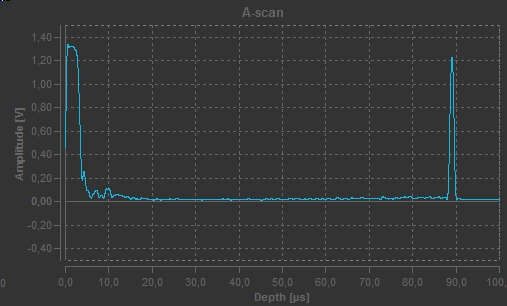
\includegraphics{Bilder/a.pdf}
	\caption{Durchbiegung $D(x)$ des Aluminiumstabes aufgetragen gegen $L_{\mathrm{eckig}}x^2-\frac{x^3}{3}$}
	\label{fig:alu_einseitig}
\end{figure}
Für den Parameter $a$ ergibt sich
\begin{equation*}
	a=(64.16\pm 0.20) \,\si{\per\square\meter}  \text{.}
\end{equation*}
Aus Gleichung \eqref{eqn:d_x_einseitig} ergibt sich der Zusammenhang

\begin{equation}
	a= \frac{F}{2EI}=\frac{m_{\mathrm{Last}}g}{2EI} \rightarrow E=\frac{m_{\mathrm{Last}}g}{2I\cdot a}
\end{equation}
Für das Flächenträgheitsmoment $I$ ergibt sich nach \cite{bla}
\begin{equation}
	I_{\mathrm{eckig}}=\frac{a_{\mathrm{eckig}}^4}{12}= 8.34 \cdot 10^{-10} \,\si{\meter\tothe{4}}	 \text{.}
\end{equation}
Mit der Erdanziehung $g=(9.811899 \pm 0.000041) \,\si{\meter\per\square\second}$ (für Dortmund) nach \cite{G} und der Masse der Last $m_{\mathrm{Last}}=767.4\,\si{\gram}$ ergibt sich der Elastizitätsmodul zu
\begin{equation*}
	E_{\mathrm{alu}}= (70.42 \pm 0.22)\,\si{\giga\pascal} \text{.}
\end{equation*}
%%%%%%%%%%%%%%%%%%%%%%%%%%%%%%%%%%%%%%%%%%%%%%%%%%%%%%%%%%%%%%%%%%%
\FloatBarrier
\subsection{Durchbiegung des runden Stabs (Messing) bei einseitiger Einspannung}
Der Elastizitätsmodul für den Messingsstab ergibt sich nach dem gleichen Prinzip wie beim Aluminiumstab.
Die Messpunkte im Abstand $x$ von der Einspannung samt den zugehörigen Auslenkungen ohne Belastung $D_{\mathrm{0}}$
und der Auslenkung mit angehängtem Gewicht $D_{\mathrm{M}}$ sowie der Differenz $D(x)$ finden sich in Tabelle \ref{tab:b}.

\begin{longtable}[c]{cccc}
	\caption{Messergebnisse für die Durchbiegung des Messingstabs bei einseitiger Einspannung.}\\
	\label{tab:b}\\
	\toprule
	$x$ /$\si{\centi\meter}$ & $D_{\mathrm{0}}$/$\si{\milli\meter}$ & $D_{\mathrm{M}}$/$\si{\milli\meter}$ & $D(x)$/$\si{\milli\meter}$ \\

	\midrule
	\endfirsthead
	\caption{Fortsetzung: Messergebnisse für die Durchbiegung des Messingstabs bei einseitiger Einspannung.}\\
	\midrule
	$x$ /$\si{\centi\meter}$ & $D_{\mathrm{0}}$/$\si{\milli\meter}$ & $D_{\mathrm{M}}$/$\si{\milli\meter}$ & $D(x)$/$\si{\milli\meter}$ \\

	\midrule
	\endhead
	\midrule
	\multicolumn{4}{r}{Weiter auf der nächsten Seite}\\
	\midrule
	\endfoot
	\bottomrule

	\endlastfoot
	3                        & 0.00                                 & 0.08                                 & 0.08                       \\
	4                        & -0.04                                & 0.05                                 & 0.09                       \\
	5                        & -0.05                                & 0.07                                 & 0.12                       \\
	6                        & -0.09                                & 0.10                                 & 0.19                       \\
	7                        & -0.10                                & 0.12                                 & 0.22                       \\
	8                        & -0.13                                & 0.12                                 & 0.25                       \\
	9                        & -0.17                                & 0.19                                 & 0.36                       \\
	10                       & -0.17                                & 0.24                                 & 0.41                       \\
	11                       & -0.18                                & 0.32                                 & 0.50                       \\
	12                       & -0.19                                & 0.39                                 & 0.58                       \\
	13                       & -0.19                                & 0.44                                 & 0.63                       \\
	14                       & -0.18                                & 0.52                                 & 0.70                       \\
	15                       & -0.18                                & 0.60                                 & 0.78                       \\
	16                       & -0.19                                & 0.73                                 & 0.92                       \\
	17                       & -0.16                                & 0.79                                 & 0.95                       \\
	18                       & -0.20                                & 0.89                                 & 1.09                       \\
	19                       & -0.19                                & 1.01                                 & 1.20                       \\
	20                       & -0.19                                & 1.20                                 & 1.39                       \\
	21                       & -0.18                                & 1.28                                 & 1.46                       \\
	22                       & -0.17                                & 1.38                                 & 1.55                       \\
	23                       & -0.13                                & 1.50                                 & 1.63                       \\
	24                       & -0.13                                & 1.63                                 & 1.76                       \\
	25                       & -0.11                                & 1.79                                 & 1.90                       \\
	26                       & -0.07                                & 1.91                                 & 1.98                       \\
	27                       & -0.07                                & 2.05                                 & 2.12                       \\
	28                       & -0.05                                & 2.22                                 & 2.27                       \\
	29                       & -0.03                                & 2.37                                 & 2.40                       \\
	30                       & -0.01                                & 2.54                                 & 2.55                       \\
	31                       & 0.03                                 & 2.71                                 & 2.68                       \\
	32                       & 0.03                                 & 2.84                                 & 2.81                       \\
	33                       & 0.06                                 & 2.97                                 & 2.91                       \\
	34                       & 0.06                                 & 3.12                                 & 3.06                       \\
	35                       & 0.07                                 & 3.30                                 & 3.23                       \\
	36                       & 0.08                                 & 3.47                                 & 3.39                       \\
	37                       & 0.11                                 & 3.65                                 & 3.54                       \\
	38                       & 0.13                                 & 3.81                                 & 3.68                       \\
	39                       & 0.15                                 & 3.98                                 & 3.83                       \\
	40                       & 0.18                                 & 4.14                                 & 3.96                       \\
	41                       & 0.24                                 & 4.30                                 & 4.06                       \\
	42                       & 0.24                                 & 4.57                                 & 4.33                       \\
	43                       & 0.29                                 & 4.66                                 & 4.37                       \\
	44                       & 0.30                                 & 4.83                                 & 4.53                       \\
	45                       & 0.35                                 & 5.01                                 & 4.66                       \\
	46                       & 0.41                                 & 5.20                                 & 4.79                       \\
	47                       & 0.42                                 & 5.45                                 & 5.03                       \\
	48                       & 0.47                                 & 5.58                                 & 5.11                       \\
	49                       & 0.52                                 & 5.79                                 & 5.27                       \\

\end{longtable}

Eine lineare Regression mittels Python nach Gleichung \eqref{eqn:d_x_einseitig} für $D(x)$ gegen $L_{mathrm{eckig}}x^2-\frac{x^3}{3}$
findet sich in Abbildung \ref{fig:messing_einseitig}.

\begin{figure}
	\centering
	\includegraphics{Bilder/b.pdf}
	\caption{Durchbiegung $D(x)$ des Messingstabes aufgetragen gegen $L_{\mathrm{eckig}}x^2-\frac{x^3}{3}$}
	\label{fig:messing_einseitig}
\end{figure}
Der Regressionsparameter wird erneut zur Berechnung von $E$ verwendet.
Es ergibt sich
\begin{equation*}
	a=(69.48 \pm 0.39) \,\si{\per\square\meter} \text{.}
\end{equation*}
Mit Gleichung \eqref{eqn:d_x_einseitig} ergibt sich
\begin{equation}
	E=\frac{m_{\mathrm{Last}}g}{2I\cdot a} \text{.}
\end{equation}
Mit \cite{bla} ergibt sich für das Flächenträgheitsmoment
\begin{equation}
	I_{\mathrm{rund}}=\frac{d_{\mathrm{rund}}^2}{16}= 4.91 \cdot 10^{-10} \,\si{\meter\tothe{4}}	 \text{.}
\end{equation}
Mit der Erdanziehung $g=(9.811899 \pm 0.000041) \,\si{\meter\per\square\second}$ nach \cite{G} und der Masse der Last $m_{\mathrm{Last}}=520.9\,\si{\gram}$ ergibt sich der Elastizitätsmodul zu
\begin{equation*}
	E_{\mathrm{Messing}}= (74.9 \pm 0.4)\,\si{\giga\pascal} \text{.}
\end{equation*}

%%%%%%%%%%%%%%%%%%%%%%%%%%%%%%%%%%%%%%%%%%%%%%%%%%%%%%%%%%%%%%%%%%%%%%%%%%%%%%%%%%%%
\FloatBarrier
\subsection{Durchbiegung des Stabes bei beidseitiger Einspannung}

Die Messwerte zur beidseitigen Einspannung sind in Tabelle \ref{tab:beidi} aufgetragen.


\begin{longtable}[c]{cccc}
	\caption{Messergebnisse für die Durchbiegung eines Stabes bei beidseitiger Einspannung.}\\
	\label{tab:beidi}\\
	\toprule
	$x$ / $\si{\centi\meter}$ & $D_0(x)$ / $\si{\milli\meter}$ & $D_{\mathrm{M}}(x)$ / $\si{\milli\meter}$ & $D(x)$ / $\si{\milli\meter}$ \\
	\midrule
	\endfirsthead
	\caption{Fortsetzung: Messergebnisse für die Durchbiegung eines Stabes bei beidseitiger Einspannung.}\\
	\midrule
	$x$ / $\si{\centi\meter}$ & $D_0(x)$ / $\si{\milli\meter}$ & $D_{\mathrm{M}}(x)$ / $\si{\milli\meter}$ & $D(x)$ / $\si{\milli\meter}$ \\
	\midrule
	\endhead
	\midrule
	\multicolumn{4}{r}{Weiter auf der nächsten Seite}\\
	\midrule
	\endfoot
	\bottomrule

	\endlastfoot
	0                         & 1.00                           & 1.09                                      & 0.09                         \\
	1                         & 0.99                           & 1.23                                      & 0.24                         \\
	2                         & 0.98                           & 1.38                                      & 0.40                         \\
	3                         & 0.96                           & 1.52                                      & 0.56                         \\
	4                         & 0.97                           & 1.68                                      & 0.71                         \\
	5                         & 0.96                           & 1.84                                      & 0.88                         \\
	6                         & 0.96                           & 1.97                                      & 1.01                         \\
	7                         & 0.95                           & 2.12                                      & 1.17                         \\
	8                         & 0.97                           & 2.26                                      & 1.29                         \\
	9                         & 0.95                           & 2.40                                      & 1.45                         \\
	10                        & 0.95                           & 2.53                                      & 1.58                         \\
	11                        & 0.93                           & 2.64                                      & 1.71                         \\
	12                        & 0.93                           & 2.77                                      & 1.84                         \\
	13                        & 0.93                           & 2.90                                      & 1.97                         \\
	14                        & 0.91                           & 3.00                                      & 2.09                         \\
	15                        & 0.90                           & 3.09                                      & 2.19                         \\
	16                        & 0.89                           & 3.19                                      & 2.30                         \\
	17                        & 0.88                           & 3.28                                      & 2.40                         \\
	18                        & 0.86                           & 3.35                                      & 2.49                         \\
	19                        & 0.84                           & 3.42                                      & 2.58                         \\
	20                        & 0.83                           & 3.48                                      & 2.65                         \\
	21                        & 0.81                           & 3.53                                      & 2.72                         \\
	22                        & 0.79                           & 3.58                                      & 2.79                         \\
	23                        & 0.78                           & 3.60                                      & 2.82                         \\
	24                        & 0.70                           & 3.64                                      & 2.94                         \\
	25                        & 0.70                           & 3.65                                      & 2.95                         \\
	26                        & 0.67                           & 3.65                                      & 2.98                         \\
	27                        & 0.65                           & --                                        & --                           \\
	28                        & 1.48                           & 4.41                                      & 2.93                         \\
	29                        & 1.46                           & 4.38                                      & 2.92                         \\
	30                        & 1.44                           & 4.34                                      & 2.90                         \\
	31                        & 1.41                           & 4.29                                      & 2.88                         \\
	32                        & 1.40                           & 4.22                                      & 2.82                         \\
	33                        & 1.38                           & 4.15                                      & 2.77                         \\
	34                        & 1.35                           & 4.06                                      & 2.71                         \\
	35                        & 1.33                           & 3.96                                      & 2.63                         \\
	36                        & 1.31                           & 3.85                                      & 2.54                         \\
	37                        & 1.28                           & 3.73                                      & 2.45                         \\
	38                        & 1.26                           & 3.61                                      & 2.35                         \\
	39                        & 1.23                           & 3.49                                      & 2.26                         \\
	40                        & 1.25                           & 3.37                                      & 2.12                         \\
	41                        & 1.18                           & 3.25                                      & 2.07                         \\
	42                        & 1.17                           & 3.10                                      & 1.93                         \\
	43                        & 1.15                           & 2.95                                      & 1.80                         \\
	44                        & 1.14                           & 2.80                                      & 1.66                         \\
	45                        & 1.12                           & 2.64                                      & 1.52                         \\
	46                        & 1.11                           & 2.49                                      & 1.38                         \\
	47                        & 1.09                           & 2.34                                      & 1.25                         \\
	48                        & 1.08                           & 2.19                                      & 1.11                         \\
	49                        & 1.09                           & 2.02                                      & 0.93                         \\
	50                        & 1.06                           & 1.85                                      & 0.79                         \\
	51                        & 1.05                           & 1.70                                      & 0.65                         \\
	52                        & 1.05                           & 1.54                                      & 0.49                         \\
\end{longtable}

\begin{figure}
	\centering
	\includegraphics{Bilder/c.pdf}
	\caption{Durchbiegung der Stäbe.}
	\label{fig:Stabus}
\end{figure}

Die Durchbiegung $D(x)$ an den Orten $0 \leq x \leq \frac{L}{2}$
also $\SI{0}{\centi\meter} \leq x \leq \SI{26}{\centi\meter}$
ist in Abbildung \ref{fig:Stabus} gemäß Formel \eqref{eqn:d_x_beidseitig_eins} gegen das
Polynom $3L^2x - 4x^3$ aufgetragen.

Die Regressionsgerade der Form
\begin{equation*}
	D(x) = a \cdot x \mathrm{,}
\end{equation*}
mit $a = \frac{F}{48EI}$ gemäß Formel \eqref{eqn:d_x_beidseitig_eins}, wurde mit Scipy
\cite{scipy} berechnet.
Der Parameter $a$ ergibt sich zu
\begin{equation*}
	a = 19,61 \pm 0,08 \mathrm{.}
\end{equation*}
Damit erhält man den Elastizitätsmodul $E$ zu
\begin{equation*}
	E = (5,903 \pm 0,025) \, \si{\giga\pascal} \mathrm{.}
\end{equation*}
%%%%%%%%%%%%%%%%%%%%%%%%%%%%%%%%%%%%%%%%%%%%%%%%%%%%%%%%%%%%%%%%%%%%%%%%%%%%%%%%%%%%%%%%%%%
\begin{figure}
	\centering
	\includegraphics{Bilder/c2.pdf}
	\caption{Durchbiegung der Stäbe amk.}
	\label{fig:StabusMaximus}
\end{figure}

Die Regeressionsgerade für die zweite Hälfte des beidseitig eingespannten Stabes  mit den
zugehörigen Messwerten ist in Abbildung \ref{fig:StabusMaximus} dargestellt.
Für die Steigung der $a$ der Regressionsgerade ergibt sich
%Werte haben sich etwas geändert. Grade zu Faul zum einfügen
params 17.1770473811 und +/- 0.0826322144696
E alu= (6.741+/-0.032)e+10
params 16.2478217063 fehler 0.101296778093
E alu= (7.13+/-0.04)e+10

\begin{equation*}
	a = 20,79 \pm 0,30  \mathrm{.}
\end{equation*}
Damit erhält man für den Elastizitätsmodul $E$ den Wert
\begin{equation*}
	E = (5,57 \pm 0,08) \, \si{\giga\pascal} \mathrm{.}
\end{equation*}
